\section{Le maillage}

\subsection{Les noeuds}

\begin{remark*}
    
    Les fonctions des questions 5, 7, 9, 11, 22, 28(b) et 28(c) sont incluses dans le code fourni de l'\hyperref[sec:fonctions]{annexe B}.
    
\end{remark*}

\subsubsection{Numérotation de tous les noeuds}

\begin{reponse}{6}

\begin{center}
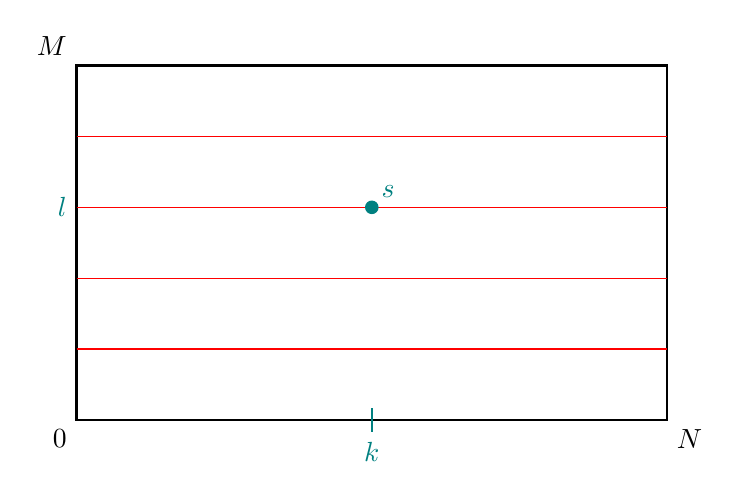
\begin{tikzpicture}[scale=1.5]
    \draw[thick] (0,0) rectangle (5,3);
    \node[below left] at (0,0) {$0$};
    \node[below right] at (5,0) {$N$};
    \node[above left] at (0,3) {$M$};
    \draw[red] (0, 0.6) -- (5, 0.6);
    \draw[red] (0, 1.2) -- (5, 1.2);
    \draw[red] (0, 1.8) -- (5, 1.8);
    \draw[red] (0, 2.4) -- (5, 2.4);
    \node[left, text=teal] at (0, 1.8) {$l$};
    \draw[thick, teal] (2.5, 0.1) -- (2.5, -0.1) node[below] {$k$};
    \filldraw[teal] (2.5, 1.8) circle (1.5pt) node[above right] {$s$};
\end{tikzpicture}
\end{center}

On a $s = l(N+1)+k$ où $l(N+1)$ représente le nombre de points sur les $l$ premières lignes et $k$ représente le nombre de points que l'on compte sur la $(l+1)$-ème ligne pour arriver à $s$.
\end{reponse}

%%%%%%%%%%%%%%%%%%%%%%%%%%%%%%%%%%%%%%%%%%%%%%%%%%%%%%%%%%%%%%%%%%%%%%%%%%%%%%%%

\begin{reponse}{8}

Soit $s \in \{ \, 0, \cdots, (N+1)(M+1)-1 \, \}$. On effectue la division euclidienne de $s$ par $N+1 \, ( \, >0 \, )$. On obtient alors :

\[
    s = (N+1) \, q + r, \quad \text{avec} \quad r < N+1.
\]

De plus, $s < (N+1)(M+1)$ donc $q < M+1$. En posant $j=q$ et $r=i$, on a l'existence. L'unicité vient de l'unicité de la division euclidienne.     
\end{reponse}

\subsection{La triangulation}

\subsubsection{Une partition en triangles}

\begin{reponse}{10}

Pour illustrer la situation, nous avons décidé de poser $N=4$ et $M=3$, pour un total de $K=24$ triangles.

\begin{center}
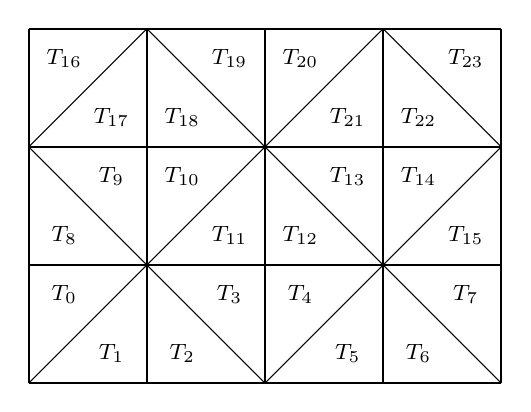
\begin{tikzpicture}[scale=1.5]
    \draw[step=1cm, thick] (0,0) grid (4,3);
    \foreach \y in {0,1,2} {
        \foreach \x in {0,1,2,3} {
            \pgfmathtruncatemacro{\cellnum}{\y*4 + \x}
            \pgfmathtruncatemacro{\tbase}{\cellnum * 2}
            \pgfmathtruncatemacro{\tplus}{\tbase + 1}
            \pgfmathtruncatemacro{\parity}{mod(\x+\y,2)}
            \ifnum\parity=0
                \draw (\x, \y) -- (\x+1, \y+1);
                \node at (\x+0.3, \y+0.75) {\footnotesize $T_{\tbase}$};
                \node at (\x+0.7, \y+0.25) {\footnotesize $T_{\tplus}$};
            \else
                \draw (\x, \y+1) -- (\x+1, \y);
                \node at (\x+0.3, \y+0.25) {\footnotesize $T_{\tbase}$};
                \node at (\x+0.7, \y+0.75) {\footnotesize $T_{\tplus}$};
            \fi
        }
    }
\end{tikzpicture}
\end{center}

\end{reponse}

\subsubsection{Coordonnées barycentriques dans un triangle. Triangle de référence}

\begin{reponse}{12}

Soit $g : x \longmapsto f(x) - f(0)$ une application de $\mathbb{R}^n$ dans $\mathbb{R}^m$. Supposons que $f$ est affine. Alors,

\[
    \forall \, x,y \in \mathbb{R}^n, \quad \forall \, \alpha \in \mathbb{R}, \quad f(\alpha x + (1- \alpha) \, y) = \alpha f(x) + (1- \alpha) \, f(y).
\]

Alors d'une part, si $\lambda \in \mathbb{R}$,

\begin{align*}
    g(\lambda x) & = f(\lambda x + (1-\lambda) \, 0) - f(0) \\
    & = \lambda f(x) + (1- \lambda) f(0) \\
    & = \lambda \, (f(x)-f(0)) = \lambda g(x),
\end{align*}

et d'autre part, 

\begin{align*}
    g(x+y) & =2g\left(\frac{1}{2} x+\frac{1}{2}y\right) \\
    & = 2\left( \frac{1}{2} f(x) + \frac{1}{2}f(y) - f(0) \right) \\
    & = f(x) + f(y)- f(0) = g(x) + g(y).
\end{align*}

Par suite, $g$ est linéaire. Réciproquement, supposons que $g$ est linéaire. Comme $g(x)=f(x)-f(0)$, on en déduit que $f(x) = g(x) - f(0)$. Ainsi, 

\begin{align*}
    f(\alpha x + (1- \alpha ) \, y) = & g(\alpha x + (1- \alpha ) \, y) + f(0) \\
    & = \alpha g(x) + (1- \alpha) \, g(y) + f(0) \\
    & = \alpha (f(x)-f(0))+f(y)-f(0)-\alpha (f(y)-f(0))+f(0) \\
    & = \alpha f(x) + (1- \alpha) \, f(y).
\end{align*}

$f$ est donc affine et cela permet de conclure.

\end{reponse}

%%%%%%%%%%%%%%%%%%%%%%%%%%%%%%%%%%%%%%%%%%%%%%%%%%%%%%%%%%%%%%%%%%%%%%%%%%%%%%%%

\begin{reponse}{13}

Comme vu à la question précédente, $f : \mathbb{R}^2 \longrightarrow \mathbb{R}$ est affine si et seulement si 

\[
    g : \mathbb{R}^2 \longrightarrow \mathbb{R}, \quad (x,y) \longmapsto f(x,y) - f(0,0)
\]

est linéaire. Si $g$ est une forme linéaire, alors elle s'écrit avec une matrice ligne de taille $1 \times 2$. On en déduit directement qu'il existe $\alpha, \beta$ deux réels tels que 

\[
    \forall \, (x,y) \in \mathbb{R}^2, \quad g(x,y) = \alpha x + \beta y.
\]

On a donc 

\[
    g(x,y) = f(x,y) - f(0,0) \quad  \Longleftrightarrow \quad \alpha x + \beta y = f(x,y) - f(0,0).
\]

Finalement, on a bien $f(x,y) = \alpha x + \beta y + \gamma$, où $\gamma = f(0,0)$.
    
\end{reponse}

%%%%%%%%%%%%%%%%%%%%%%%%%%%%%%%%%%%%%%%%%%%%%%%%%%%%%%%%%%%%%%%%%%%%%%%%%%%%%%%%

\begin{reponse}{14}
Puisque $A_0, A_1$ et $A_2$ ne sont pas alignés, les vecteurs $\overset{\rightarrow}{A_0A_1}$ et $\overset{\rightarrow}{A_0A_2}$ forment une base de $\mathbb{R}^2$. Par suite, le vecteur $\overset{\rightarrow}{A_0M}$ se décompose de manière unique dans cette base :

\[
    \overset{\rightarrow}{A_0M} = \alpha \overset{\rightarrow}{A_0A_1} + \beta \overset{\rightarrow}{A_0A_2}.
\]

On en déduit que 

\begin{align*}   
    M = A_0 + \overset{\rightarrow}{A_0M} \quad \Longleftrightarrow \quad M-A_0 & = \overset{\rightarrow}{A_0M} \\
    & = \alpha \overset{\rightarrow}{A_0A_1} + \beta \overset{\rightarrow}{A_0A_2} \\
    & = \alpha \, (A_1 - A_0) + \beta \, (A_2 - A_0) \\
    & = (-\alpha - \beta) \, A_0 + \alpha A_1 + \beta A_2.
\end{align*}

On a donc finalement que $M= (1-\alpha - \beta) \, A_0 + \alpha A_1 + \beta A_2$. On en déduit alors que 

\[
    \lambda_0(x,y) = 1-\alpha-\beta, \quad \lambda_1(x,y) = \alpha, \quad \lambda_2(x,y) = \beta
\]

et leur somme vaut bien $1$.
    
\end{reponse}

%%%%%%%%%%%%%%%%%%%%%%%%%%%%%%%%%%%%%%%%%%%%%%%%%%%%%%%%%%%%%%%%%%%%%%%%%%%%%%%%

\begin{reponse}{15}
Soit $f_i : (x,y) \longmapsto \lambda_i(x,y)$. On veut montrer que $f_i$ est de la forme $\alpha x + \beta y + \gamma $. D'après la question 14, on a le système

\[
\begin{cases}
    x = \lambda_0x_0+\lambda_1x_1 + \lambda_2x_2 \\
    y= \lambda_0y_0+\lambda_1y_1 + \lambda_2y_2 \\
    1 = \lambda_0+\lambda_1+\lambda_2
\end{cases}
\]

qui se traduit par le système matriciel suivant :

$$
\underbrace{
\begin{pmatrix}
    x_0 & x_1 & x_2 \\
    y_0 & y_1 & y_2 \\
    1 & 1 & 1
\end{pmatrix}}_{A} \begin{pmatrix}
    \lambda_0 \\
    \lambda_1 \\
    \lambda_2
\end{pmatrix} =\begin{pmatrix}
    x \\
    y \\
    1
\end{pmatrix}.
$$

De plus, 

$$
\det(A) = 
\begin{vmatrix}
    x_0 & x_1 & x_2 \\
    y_0 & y_1 & y_2 \\
    1 & 1 & 1
\end{vmatrix} = \begin{vmatrix}
    x_0 & x_1-x_0 & x_2-x_0 \\
    y_0 & y_1-y_0 & y_2-y_0 \\
    1 & 0 & 0
\end{vmatrix} = \begin{vmatrix}
    x_1-x_0 & x_2-x_0 \\
    y_1-y_0 & y_2-y_0 \\
\end{vmatrix}.
$$

Comme $$
\begin{pmatrix}
    x_1-x_0 \\
    y_1-y_0\\
\end{pmatrix} = \overset{\rightarrow}{A_0A_1}.
$$ et $$
\begin{pmatrix}
    x_2-x_0 \\
    y_2-y_0\\
\end{pmatrix} = \overset{\rightarrow}{A_0A_2}$$ et que $\overset{\rightarrow}{A_0A_1}$ et $\overset{\rightarrow}{A_0A_2}$ forment une base de $\mathbb{R}^2$, on en déduit que $A$ est inversible. Ainsi,

$$
\begin{pmatrix}
    \lambda_0 \\
    \lambda_1 \\
    \lambda_2
\end{pmatrix} =A^{-1} \begin{pmatrix}
    x \\
    y \\
    1
\end{pmatrix}$$.

Finalement, 

\[
    \lambda_i = \alpha_i x_i + \beta_i y_i + \gamma_i.
\]

On conclut grâce à la question 13 que $f_i$ est affine.

\end{reponse}

%%%%%%%%%%%%%%%%%%%%%%%%%%%%%%%%%%%%%%%%%%%%%%%%%%%%%%%%%%%%%%%%%%%%%%%%%%%%%%%%

\begin{reponse}{16}

Soit $i \in \{ \, 0,1,2 \, \}$. On a 

$$
\begin{pmatrix}
    x_i \\
    y_i
\end{pmatrix} = \delta_{0,i} \begin{pmatrix}
    x_0 \\
    y_0
\end{pmatrix} + \delta_{1,i} \begin{pmatrix}
    x_1 \\
    y_1
\end{pmatrix} + \delta_{2,i} \begin{pmatrix}
    x_2 \\
    y_2
\end{pmatrix}.
$$

On en déduit directement que $\lambda_j(x_i,y_i)= \delta_{i,j}$.
\end{reponse}

%%%%%%%%%%%%%%%%%%%%%%%%%%%%%%%%%%%%%%%%%%%%%%%%%%%%%%%%%%%%%%%%%%%%%%%%%%%%%%%%

\begin{reponse}{17}

Soit $f$ une application affine de $\mathbb{R}^2$ dans $\mathbb{R}$. Soient $\alpha, \beta,\gamma \in \mathbb{R}$ tels que pour tout $(x,y) \in \mathbb{R}^2$, 

\[
    f(x,y) = \alpha x + \beta y + \gamma.
\]

D'après la question 14, on a :

\begin{align*}  
    f(x,y) & = \alpha \, (\lambda_0x_0 + \lambda_1x_1+\lambda_2x_2) + \beta \, (\lambda_0y_0 + \lambda_1y_1+\lambda_2y_2 + \gamma \, (\lambda_0+\lambda_1+\lambda_2) \\
    & = \lambda_0 \, (\alpha x_0 + \beta y_0 + \gamma) + \lambda_1 \, (\alpha x_1 + \beta y_1 + \gamma) + \lambda_2 \, (\alpha x_2 + \beta y_2 + \gamma) \\
    & = \sum_{i=0}^2 f(x_i,y_i) \lambda_i.
\end{align*}

Si pour tout $i \in \{ \, 0,1,2 \, \}$, $f(x_i,y_i)=0$, alors

\[ 
    f(x,y) = \sum_{i=0}^2 0 \cdot \lambda_i(x,y) = 0 \quad \text{pour tout } (x,y) \in \mathbb{R}^2.
\]
\end{reponse}

%%%%%%%%%%%%%%%%%%%%%%%%%%%%%%%%%%%%%%%%%%%%%%%%%%%%%%%%%%%%%%%%%%%%%%%%%%%%%%%%

\begin{reponse}{18}

\begin{center}
\begin{tikzpicture}[scale=3] 
    \draw[->, gray] (-0.3, 0) -- (1.5, 0) node[right, black] {$x$};
    \draw[->, gray] (0, -0.3) -- (0, 1.5) node[above, black] {$y$};
    \draw[thick, black] (0,0) -- (1,0) -- (0,1) -- cycle;
    \filldraw (0,0) circle (0.5pt) node[below left] {$\hat{A}_0(0,0)$};
    \filldraw (1,0) circle (0.5pt) node[below] {$\hat{A}_1(1,0)$};
    \filldraw (0,1) circle (0.5pt) node[left] {$\hat{A}_2(0,1)$};
    \node at (0.3, 0.3) {$\hat{T}$};
\end{tikzpicture}
\end{center}

Soit $(x,y) \in \mathbb{R}^2$. Alors de $$\begin{pmatrix}
    x \\
    y
\end{pmatrix} = \hat{\lambda_0} \begin{pmatrix}
    0\\0
\end{pmatrix} + \hat{\lambda_1}\begin{pmatrix}
    1\\0
\end{pmatrix} + \hat{\lambda_2}\begin{pmatrix}
    0\\1
\end{pmatrix},$$ on déduit que $\hat{\lambda_1}=x$ et $\hat{\lambda_2}=y$. Comme de plus la somme des $\hat{\lambda_i}$ fait $1$, alors $\hat{\lambda_0} = 1-x-y$.
\end{reponse}

%%%%%%%%%%%%%%%%%%%%%%%%%%%%%%%%%%%%%%%%%%%%%%%%%%%%%%%%%%%%%%%%%%%%%%%%%%%%%%%%

\begin{reponse}{19}

Posons l'application $F_T : \mathbb{R}^2 \to \mathbb{R}^2$ définie par :
\begin{align*}
    F_T(\hat{x}, \hat{y}) & = \hat{\lambda}_0(\hat{x}, \hat{y}) A_0 + \hat{\lambda}_1(\hat{x}, \hat{y}) A_1 + \hat{\lambda}_2(\hat{x}, \hat{y}) A_2 \\
    & = (1 - \hat{x} - \hat{y}) A_0 + \hat{x} A_1 + \hat{y} A_2 \\ 
    & = A_0 + \hat{x}(A_1 - A_0) + \hat{y}(A_2 - A_0).
\end{align*}
où les $A_i$ sont les sommets du triangle $T$. On reconnaît que $F_T$ s'écrit comme la somme d'un vecteur constant $A_0$ et d'une combinaison linéaire des variables $(\hat{x}, \hat{y})$ avec les vecteurs constants $\overset{\rightarrow}{A_0A_1}$ et $\overset{\rightarrow}{A_0A_2}$. L'application $F_T$ est donc bien une transformation affine. De plus, elle transforme bien les sommets de $\hat{T}$ en ceux de $T$. En effet, D'après la question 16, on sait que $\hat{\lambda}_i(\hat{A}_j) = \delta_{ij}$ (où $\delta_{ij}$ vaut $1$ si $i=j$ et $0$ sinon). On a donc :

\[
    F_T(\hat{A}_j) = \sum_{i=0}^2 \hat{\lambda}_i(\hat{A}_j) A_i = A_j
\]

Il s'agit désormais de montrer l'unicité de $F_T$. Posons $F_T(\hat{x}, \hat{y}) = \begin{pmatrix}
    f_1(\hat{x}, \hat{y}) \\ f_2(\hat{x}, \hat{y})
\end{pmatrix}$. Comme $f_1$ est une application de $\mathbb{R}^2 \longrightarrow \mathbb{R}$, alors par la question 17, elle est uniquement définie par les valeurs aux sommets de $\hat{T}$. De la même manière, $f_2$ est aussi uniquement définie par les valeurs aux sommets de $\hat{T}$. Les composantes $f_1$ et $f_2$ étant définies de façon unique par les coordonnées des sommets $A_i$, la transformation $F_T$ est elle-même unique.

\end{reponse}

%%%%%%%%%%%%%%%%%%%%%%%%%%%%%%%%%%%%%%%%%%%%%%%%%%%%%%%%%%%%%%%%%%%%%%%%%%%%%%%%

\begin{reponse}{20}

Montrons que $F_T$ est inversible. Posons $F_T(X)=B_TX+C$, où $C$ est un vecteur de $\mathbb{R}^2$ et $B_T$ une matrice $2 \times 2$ à coefficients réels qui représente la partie linéaire de $F_T$. Alors $F_T$ est inversible si et seulement si $B_T$ est inversible. Par définition de $F_T$, nous avons le système suivant : 

\[
    \begin{cases}
        F_T(\hat{A_0})=A_0 \\ F_T(\hat{A_1})=A_1 \\ F_T(\hat{A_2})=A_2
    \end{cases}. 
\]

Dans le triangle $\hat{T}$, les points ont pour coordonnées $\hat{A_0}(0,0)$, $\hat{A_1}(1,0)$ et $\hat{A_2}(0,1)$. Les vecteurs $\overset{\rightarrow}{\hat{A_0}\hat{A_1}}$ et $\overset{\rightarrow}{\hat{A_0}\hat{A_2}}$ ont donc pour coordonnées respectives $$\begin{pmatrix}
    1 \\ 0
\end{pmatrix} \quad \text{et} \quad \begin{pmatrix}
    0 \\ 1
\end{pmatrix},$$ ce qui correspond à la base canonique de $\mathbb{R}^2$. Par linéarité de $B_T$, on obtient :

\begin{align*}
    B_T(\overset{\rightarrow}{\hat{A_0}\hat{A_1}})=F_T(\hat{A_0})-F_T(\hat{A_1}) = \overset{\rightarrow}{A_0A_1} \\
    B_T(\overset{\rightarrow}{\hat{A_0}\hat{A_2}})=F_T(\hat{A_0})-F_T(\hat{A_2}) = \overset{\rightarrow}{A_0A_2}
\end{align*}.

Dans la base canonique, on a donc :

\[
    B_T = \left( \overset{\rightarrow}{A_0A_1} \quad \overset{\rightarrow}{A_0A_2} \right).
\]

Or comme vu à la question 14, les vecteurs $\overset{\rightarrow}{A_0A_1}$ $\overset{\rightarrow}{A_0A_2}$ forment une base de $\mathbb{R}^2$. Par suite, $B_T$ est inversible et donc $F_T$ l'est également.
\end{reponse}

%%%%%%%%%%%%%%%%%%%%%%%%%%%%%%%%%%%%%%%%%%%%%%%%%%%%%%%%%%%%%%%%%%%%%%%%%%%%%%%%

\begin{reponse}{21}

Soit $F_T(\hat{x}, \hat{y}) = (f_1(\hat{x}, \hat{y}), f_2(\hat{x}, \hat{y}))$ la transformation affine de $\mathbb{R}^2$ dans $\mathbb{R}^2$ qui transforme le triangle de référence $\hat{T}$ en $T$. En utilisant les fonctions coordonnées barycentriques $\hat{\lambda}_0$, $\hat{\lambda}_1$ et $\hat{\lambda}_2$ du triangle de référence $\hat{T}$, on peut exprimer l'image d'un point par $F_T$ comme combinaison affine des sommets $A_0(x_0, y_0)$, $A_1(x_1, y_1)$ et $A_2(x_2, y_2)$ :
$$F_T(\hat{x}, \hat{y}) = \hat{\lambda}_0(\hat{x}, \hat{y})A_0 + \hat{\lambda}_1(\hat{x}, \hat{y})A_1 + \hat{\lambda}_2(\hat{x}, \hat{y})A_2$$

Comme $\hat{\lambda}_0(\hat{x}, \hat{y}) = 1 - \hat{x} - \hat{y}$, $\hat{\lambda}_1(\hat{x}, \hat{y}) = \hat{x}$ et $\hat{\lambda}_2(\hat{x}, \hat{y}) = \hat{y}$, on a :
$$F_T(\hat{x}, \hat{y}) = (1 - \hat{x} - \hat{y}) \begin{pmatrix} x_0 \\ y_0 \end{pmatrix} + \hat{x} \begin{pmatrix} x_1 \\ y_1 \end{pmatrix} + \hat{y} \begin{pmatrix} x_2 \\ y_2 \end{pmatrix}$$

En séparant les composantes $f_1$ et $f_2$, on obtient :

\begin{align*}
    f_1(\hat{x}, \hat{y}) = x_0 + \hat{x}(x_1 - x_0) + \hat{y}(x_2 - x_0) \\ \\
    f_2(\hat{x}, \hat{y}) = y_0 + \hat{x}(y_1 - y_0) + \hat{y}(y_2 - y_0)
\end{align*}

Par définition, la matrice jacobienne $B_T$ est :

\[
    B_T = \begin{pmatrix} \frac{\partial f_1}{\partial \hat{x}} & \frac{\partial f_1}{\partial \hat{y}} \\ \frac{\partial f_2}{\partial \hat{x}} & \frac{\partial f_2}{\partial \hat{y}} \end{pmatrix}.
\]


Les dérivées partielles sont
:

\[
    \frac{\partial f_1}{\partial \hat{x}} = x_1 - x_0, \quad \frac{\partial f_1}{\partial \hat{y}} = x_2 - x_0, \quad \frac{\partial f_2}{\partial \hat{x}} = y_1 - y_0, \quad \frac{\partial f_2}{\partial \hat{y}} = y_2 - y_0.
\]

La matrice jacobienne $B_T$ en fonction des coordonnées des sommets du triangle $T$ est donc :
$$B_T = \begin{pmatrix} x_1 - x_0 & x_2 - x_0 \\ y_1 - y_0 & y_2 - y_0 \end{pmatrix}$$
\end{reponse}

%%%%%%%%%%%%%%%%%%%%%%%%%%%%%%%%%%%%%%%%%%%%%%%%%%%%%%%%%%%%%%%%%%%%%%%%%%%%%%%%

\begin{reponse}{23}

Notons l'aire du triangle $T$ $Aire(T)$. ALors par définition, on a

\[
    Aire(T)= \int_T 1 dxdy.
\]

On effectue le changement de variable $(x,y)= F_T(\hat{x}, \hat{y})$. La formule du changement de variable nous donne :

\[
    Aire(T) = \int_{\hat{T}} \vert \det(B_T) \, \vert d\hat{x}d\hat{y}.
\]

De plus, l'aire du triangle de référence, qui est rectangle isocèle, est donnée par

\[
    Aire(\hat{T})= \frac{1 \times 1}{2} = \frac{1}{2}.
\]

On a donc finalement

\[
    Aire(T)=\frac{1}{2} \vert \det(B_T) \, \vert.
\]

\end{reponse}

%%%%%%%%%%%%%%%%%%%%%%%%%%%%%%%%%%%%%%%%%%%%%%%%%%%%%%%%%%%%%%%%%%%%%%%%%%%%%%%%

\begin{reponse}{24}

Soit $M$ un point quelconque du triangle $T$. Ses coordonnées barycentriques par rapport aux sommets $A_0$, $A_1$, et $A_2$ vérifient :

\[
    M = \lambda_0(M)A_0+\lambda_1(M)A_1 + \lambda_2(M)A_2,
\]

où $\sum_{i=0}^2 \lambda_i(M) = 1$. D'après la question 20, $F_T$ est inversible. On en déduit donc que $F_T^{-1}$ est une bijection affine qui envoie $T$ sur $\hat{T}$. Ainsi, 

\begin{align*}
    F_T^{-1}(M) & =\lambda_0(M)F_T^{-1}(A_0)+\lambda_1(M)F_T^{-1}(A_1) + \lambda_2(M)F_T^{-1}(A_2) \\
    & = \lambda_0(M)\hat{A_0}+\lambda_1(M)\hat{A_1} + \lambda_2(M)\hat{A_2}
\end{align*}

Si on note $\hat{M} = F_T^{-1}(M) \in \hat{T}$, alors les $\lambda_i(M)$ sont les coordonnées barycentriques du point $\hat{M}$ par rapport au triangle de référence $\hat{T}$. Par unicité des coordonnées barycentriques, on a donc :

\[
    \lambda_i(M) = \hat{\lambda_i}(\hat{M}) = \hat{\lambda_i}(F_T^{-1}(\hat{M})).
\]

On en déduit finalement que 

\[
    \lambda_i = \hat{\lambda_i} \circ F_T^{-1}.
\]

\end{reponse}

%%%%%%%%%%%%%%%%%%%%%%%%%%%%%%%%%%%%%%%%%%%%%%%%%%%%%%%%%%%%%%%%%%%%%%%%%%%%%%%%
\newpage

\begin{reponse}{25}

D'après la question 24, $\lambda_i = \hat{\lambda_i} \circ F_T^{-1}$. On a donc que :

\[
    \text{Jac}(\lambda_i) =  \text{Jac}(\hat{\lambda_i}) \times  \text{Jac} (F_T^{-1}),
\]

où $ \text{Jac}(f) = (\nabla f)^T$ est la jacobienne de la fonction $f$. Comme de plus $\text{Jac} (F_T^{-1}) = B_T^{-1}$ (par les questions 20 et 21), on a :

\begin{align*}
    \text{Jac}(\lambda_i) & =  \text{Jac}(\hat{\lambda_i}) \times  \text{Jac} (F_T^{-1}) \\ \\
   \Longleftrightarrow \quad & (\nabla \lambda_i)^T = (\nabla \hat{\lambda_i})^T B_T^{-1} \\ \\
   \Longleftrightarrow \quad & \nabla \lambda_i = (B_T^{-1})^T \,  \nabla \hat{\lambda_i}.
   \end{align*}
    
\end{reponse}

%%%%%%%%%%%%%%%%%%%%%%%%%%%%%%%%%%%%%%%%%%%%%%%%%%%%%%%%%%%%%%%%%%%%%%%%%%%%%%%%

\begin{reponse}{26}

On cherche à calculer $\int_T \eta \, \langle \, \nabla \lambda_k \, \vert \, \nabla \lambda_j \, \rangle \, dxdy$. D'après la question 25, $\nabla \lambda_i = (B_T^{-1})^T \,  \nabla \hat{\lambda_i}$. De plus, $\langle \, \nabla \lambda_k \, \vert \, \nabla \lambda_j \, \rangle$ est une constante. On a donc :

\[
    \int_T \eta \, \langle \, \nabla \lambda_k \, \vert \, \nabla \lambda_j \, \rangle \, dxdy  = \langle \, (B_T^{-1})^T \, \nabla \hat{\lambda_k} \, \vert \, (B_T^{-1})^T \, \nabla \hat{\lambda_j} \, \rangle \, \int_T \eta \, dxdy.
\]

Exprimons maintenant $\int_T \lambda_k \lambda_j \, dxdy$. En effectuant le changement de variables $(x,y) = F_T(\hat{x}, \hat{y})$ et en réutilisant le résultat de la question 24 selon lequel $\lambda_i(x,y) = \hat{\lambda_i}(\hat{x},\hat{y})$, on obtient :

\[
    \int_T \lambda_k \lambda_j \, dxdy = \int_{\hat{T}} \hat{\lambda_k}\hat{\lambda_j} \, \vert \det(B_T) \, \vert \, d\hat{x}d\hat{y} =  \vert \det(B_T) \, \vert \int_{\hat{T}} \hat{\lambda_k}\hat{\lambda_j} \, d\hat{x}d\hat{y}.
\]
    
\end{reponse}

%%%%%%%%%%%%%%%%%%%%%%%%%%%%%%%%%%%%%%%%%%%%%%%%%%%%%%%%%%%%%%%%%%%%%%%%%%%%%%%%

\begin{reponse}{27}

Sur le triangle de référence $\hat{T}$, les fonctions coordonnées barycentriques sont définies par :

\[
    \hat{\lambda_0}(\hat{x},\hat{y}) = 1-\hat{x}-\hat{y}, \quad \hat{\lambda_1}(\hat{x},\hat{y}) = \hat{x}, \quad \hat{\lambda_2}(\hat{x},\hat{y}) = \hat{y}.
\]

Il faut donc évaluer les 6 intégrales suivantes :

\begin{itemize}
    \item Pour $k=j=1$ :
        \begin{align*}
            \int_{\hat{T}} \hat{\lambda}_1^2 \, d\hat{x}d\hat{y}  & = \int_0^1 \int_0^{1-\hat{x}} \hat{x}^2 \, d\hat{y}d\hat{x} = \int_0^1 \hat{x}^2 (1 - \hat{x}) \, d\hat{x} \\ \\
            & = \left[ \frac{\hat{x}^3}{3} - \frac{\hat{x}^4}{4} \right]_0^1 = \frac{1}{3} - \frac{1}{4} = \frac{1}{12}
        \end{align*}
    \item Pour $k=j=2$, par symétrie :
        \[
            \int_{\hat{T}} \hat{\lambda}_2^2 \, d\hat{x}d\hat{y} = \int_0^1 \int_0^{1-\hat{y}} \hat{y}^2 \, d\hat{x}d\hat{y} = \frac{1}{12}
        \]
    \item Pour $k=j=0$ :
        \begin{align*}
            \int_{\hat{T}} \hat{\lambda}_0^2 \, d\hat{x}d\hat{y} &= \int_0^1 \int_0^{1-\hat{x}} (1 - \hat{x} - \hat{y})^2 \, d\hat{y}d\hat{x} = \int_0^1 \left[ -\frac{1}{3}(1 - \hat{x} - \hat{y})^3 \right]_0^{1-\hat{x}} \, d\hat{x} \\ \\
            &= \int_0^1 \frac{1}{3}(1 - \hat{x})^3 \, d\hat{x} = \left[ -\frac{1}{12}(1 - \hat{x})^4 \right]_0^1 = \frac{1}{12}
        \end{align*}
    \item Pour $k=1$, $j=2$ : 
        \begin{align*}
            \int_{\hat{T}} \hat{\lambda}_1 \hat{\lambda}_2 \, d\hat{x}d\hat{y} &= \int_0^1 \int_0^{1-\hat{x}} \hat{x} \hat{y} \, d\hat{y}d\hat{x} = \int_0^1 \hat{x} \left[ \frac{\hat{y}^2}{2} \right]_0^{1-\hat{x}} \, d\hat{x} = \frac{1}{2} \int_0^1 \hat{x}(1 - \hat{x})^2 \, d\hat{x} \\ \\
            &= \frac{1}{2} \int_0^1 (\hat{x} - 2\hat{x}^2 + \hat{x}^3) \, ddd\hat{x} = \frac{1}{2} \left( \frac{1}{2} - \frac{2}{3} + \frac{1}{4} \right) = \frac{1}{24}
        \end{align*}
    \item Pour $k=0$, $j=1$ :
        \begin{align*}
            \int_{\hat{T}} \hat{\lambda}_0 \hat{\lambda}_1  \, d\hat{x}d\hat{y} &= \int_0^1 \int_0^{1-\hat{x}} (1 - \hat{x} - \hat{y})\hat{x} \, d\hat{y}d\hat{x} = \int_0^1 \hat{x} \left[ (1-\hat{x})\hat{y} - \frac{\hat{y}^2}{2} \right]_0^{1-\hat{x}} \, d\hat{x} \\ \\
            &= \int_0^1 \hat{x} \left( (1-\hat{x})^2 - \frac{(1-\hat{x})^2}{2} \right) \, d\hat{x} = \frac{1}{2} \int_0^1 \hat{x}(1-\hat{x})^2 \, d\hat{x} = \frac{1}{24}
        \end{align*}
    \item Pour $k=0$, $j=2$, par symétrie :
        \begin{align*}
            \int_{\hat{T}} \hat{\lambda}_0 \hat{\lambda}_2 \, d\hat{x}d\hat{y} = \frac{1}{24}
        \end{align*}
\end{itemize}


\end{reponse}

%%%%%%%%%%%%%%%%%%%%%%%%%%%%%%%%%%%%%%%%%%%%%%%%%%%%%%%%%%%%%%%%%%%%%%%%%%%%%%%%

\begin{reponse}{28}
    \textbf{(a)} Posons $I(h) = \int_{\hat{T}} h(\hat{x},\hat{y}) \, dxdy$ l'intégrale exacte et $Q(h)$ la formule de quadrature des points milieux associés suivante :
    
    \[
        Q(h) = \frac{1}{6} \left(h\left(\frac{1}{2},0\right)+h\left(0,\frac{1}{2}\right)+h \left(\frac{1}{2},\frac{1}{2}\right)\right).
    \]
    
    Testons la méthode pour les polynômes de degrés $p+q=d$ : 
    \\
    \begin{itemize}
        \item Pour $d=0$ : \\
        Alors $h(\hat{x}, \hat{y}) = 1$. On a donc $I(1)=\frac{1}{2}$. 
        \[
            Q(1) = \frac{1}{6} \left(1 + 1 +1 \right) = \frac{1}{2}.
        \]
        La formule est donc exacte pour le degré $0$. \\
        \item Pour $d=1$ : \\
        Par symétrie, il suffit de tester $h(\hat{x},\hat{y}) = \hat{x}$.
        \[
            I(\hat{x}) = \int_0^1 \int_0^{1-\hat{x}} \hat{x} \, d\hat{y}d\hat{x} = \int_0^1 \hat{x}(1-\hat{x}) \, d\hat{x} = \left[ \frac{\hat{x}^2}{2} - \frac{\hat{x}^3}{3} \right]_0^1 = \frac{1}{6}
        \]
        \[
            Q(\hat{x}) = \frac{1}{6} \left( \frac{1}{2} +0 + \frac{1}{2} \right) = \frac{1}{6}
        \]
        La formule est donc exacte pour le degré $1$. \\
        \item Pour $d=2$ :
        Il faut tester pour les monômes $\hat{x}^2$, $\hat{y}^2$ et $\hat{x}\hat{y}$. \\
        \begin{itemize}
            \item Pour $h(\hat{x}, \hat{y}) = \hat{x}^2$ (et $\hat{y}^2$ par symétrie) :
            \[
                I(\hat{x}^2) = \frac{1}{12} \quad \text{(d'après la question 27)}.
            \]
            \[
                Q(\hat{x}^2) = \frac{1}{6}\left(\left(\frac{1}{2}\right)^2 + 0 + \left( \frac{1}{2}\right)^2 \right)= \frac{1}{6} \times \frac{1}{2} = \frac{1}{12}
            \] \\
            \item Pour $h(\hat{x}, \hat{y}) = \hat{x}\hat{y}$ :
            \[
                I(\hat{x}\hat{y}) = \frac{1}{24} \quad \text{(d'après la question 27)}
            \]
            \[
                Q(\hat{x}\hat{y}) = \frac{1}{6}\left(\frac{1}{2} \times 0 + 0 \times \frac{1}{2} + \frac{1}{2} \times \frac{1}{2}\right) = \frac{1}{6} \times \frac{1}{4} = \frac{1}{24}
            \]    
        \end{itemize}
        La formule est donc également exacte pour le degré $2$. \\
        \item Pour $d=3$ :
        On teste le monôme $h(\hat{x}, \hat{y}) = \hat{x}^3$.
        \[
            I(\hat{x}^3) = \int_0^1 \int_0^{1-\hat{x}} \hat{x}^3 \, d\hat{y}d\hat{x} = \int_0^1 \hat{x}^3(1-\hat{x}) \, d\hat{x} = \left[ \frac{\hat{x}^4}{4} - \frac{\hat{x}^5}{5} \right]_0^1 = \frac{1}{4} - \frac{1}{5} = \frac{1}{20}
        \]
        \[
            Q(\hat{x}^3) = \frac{1}{6} \left( \left(\frac{1}{2}\right)^3 + 0 + \left(\frac{1}{2}\right)^3 \right) = \frac{1}{6} \left( \frac{1}{8} + \frac{1}{8} \right) = \frac{2}{48} = \frac{1}{24}
        \]
        On observe que $I(\hat{x}^3) \neq Q(\hat{x}^3)$.
    \end{itemize} 

    \vspace{0.8em}
    
    Finalement, la première formule de quadrature est juste pour les polynômes de degré inférieur ou égal à $d=2$. Testons maintenant pour la formule de quadrature $R(h)$ donnée par :
    
    \[
        R(h) = \frac{1}{6} \left( h \left( \frac{1}{6}, \frac{1}{6}\right) + h \left(\frac{1}{6}, \frac{2}{3}\right)+ h \left( \frac{2}{3}, \frac{1}{6}\right)\right)
    \]
    
    \begin{itemize}
        \item Pour $d=0$ : \\
        Alors $h(\hat{x}, \hat{y}) = 1$. Comme précédemment, on a $I(1)=\frac{1}{2}$. 
        \[
            R(1) = \frac{1}{6} \left(1 + 1 + 1 \right) = \frac{1}{2}.
        \]
        La formule est donc exacte pour le degré $0$. \\
        \item Pour $d=1$ : \\
        Par symétrie, il suffit de tester $h(\hat{x},\hat{y}) = \hat{x}$. On a déjà calculé $I(\hat{x}) = \frac{1}{6}$.
        \[
            R(\hat{x}) = \frac{1}{6} \left( \frac{1}{6} + \frac{1}{6} + \frac{2}{3} \right) = \frac{1}{6} \left( \frac{2}{6} + \frac{4}{6} \right) = \frac{1}{6} \times 1 = \frac{1}{6}
        \]
        La formule est donc exacte pour le degré $1$. \\
        \item Pour $d=2$ :
        Il faut tester pour les monômes $\hat{x}^2$, $\hat{y}^2$ et $\hat{x}\hat{y}$. \\
        \begin{itemize}
            \item Pour $h(\hat{x}, \hat{y}) = \hat{x}^2$ (et $\hat{y}^2$ par symétrie) :
            \begin{align*}  
                R(\hat{x}^2) & = \frac{1}{6}\left(\left(\frac{1}{6}\right)^2 + \left(\frac{1}{6}\right)^2 + \left( \frac{2}{3}\right)^2 \right) \\ & = \frac{1}{6} \left( \frac{1}{36} + \frac{1}{36} + \frac{16}{36} \right) = \frac{1}{6} \times \frac{18}{36} = \frac{1}{12}
            \end{align*}
            \item Pour $h(\hat{x}, \hat{y}) = \hat{x}\hat{y}$ :
            \begin{align*}               
                R(\hat{x}\hat{y}) & = \frac{1}{6}\left(\frac{1}{6} \times \frac{1}{6} + \frac{1}{6} \times \frac{2}{3} + \frac{2}{3} \times \frac{1}{6}\right) \\ & = \frac{1}{6} \left( \frac{1}{36} + \frac{4}{36} + \frac{4}{36} \right) = \frac{1}{6} \times \frac{9}{36} = \frac{1}{24}
            \end{align*}
        \end{itemize}
    La formule est donc également exacte pour le degré $2$. \\
    \item Pour $d=3$ :
    On teste le monôme $h(\hat{x}, \hat{y}) = \hat{x}^3$. On sait d'après le calcul précédent que $I(\hat{x}^3) = \frac{1}{20}$.
    \begin{align*} 
        R(\hat{x}^3) & = \frac{1}{6} \left( \left(\frac{1}{6}\right)^3 + \left(\frac{1}{6}\right)^3 + \left(\frac{2}{3}\right)^3 \right) \\ & = \frac{1}{6} \left( \frac{1}{216} + \frac{1}{216} + \frac{64}{216} \right) = \frac{1}{6} \times \frac{66}{216} = \frac{11}{216}
    \end{align*}
    On observe que $I(\hat{x}^3) \neq R(\hat{x}^3)$.
    \end{itemize}
    
    \vspace{0.8em}

    Finalement, la deuxième formule de quadrature est également exacte pour les polynômes de degré inférieur ou égal à $d=2$.
    
\end{reponse}